\documentclass[journal,12pt,twocolumn]{IEEEtran}

\usepackage{setspace}
\usepackage{gensymb}

\singlespacing


\usepackage[cmex10]{amsmath}

\usepackage{amsthm}

\usepackage{mathrsfs}
\usepackage{txfonts}
\usepackage{stfloats}
\usepackage{bm}
\usepackage{cite}
\usepackage{cases}
\usepackage{subfig}

\usepackage{longtable}
\usepackage{multirow}


\usepackage{enumitem}
\usepackage{mathtools}
\usepackage{steinmetz}
\usepackage{tikz}
\usepackage{circuitikz}
\usepackage{verbatim}
\usepackage{tfrupee}
\usepackage[breaklinks=true]{hyperref}
\usepackage{graphicx}
\usepackage{tkz-euclide}

\usetikzlibrary{calc,math}
\usepackage{listings}
    \usepackage{color}                                            %%
    \usepackage{array}                                            %%
    \usepackage{longtable}                                        %%
    \usepackage{calc}                                             %%
    \usepackage{multirow}                                         %%
    \usepackage{hhline}                                           %%
    \usepackage{ifthen}                                           %%
    \usepackage{lscape}     
\usepackage{multicol}
\usepackage{chngcntr}
\usetkzobj{all}

\DeclareMathOperator*{\Res}{Res}

\renewcommand\thesection{\arabic{section}}
\renewcommand\thesubsection{\thesection.\arabic{subsection}}
\renewcommand\thesubsubsection{\thesubsection.\arabic{subsubsection}}

\renewcommand\thesectiondis{\arabic{section}}
\renewcommand\thesubsectiondis{\thesectiondis.\arabic{subsection}}
\renewcommand\thesubsubsectiondis{\thesubsectiondis.\arabic{subsubsection}}


\hyphenation{op-tical net-works semi-conduc-tor}
\def\inputGnumericTable{}                                 %%

\lstset{
%language=C,
frame=single, 
breaklines=true,
columns=fullflexible
}
\begin{document}


\newtheorem{theorem}{Theorem}[section]
\newtheorem{problem}{Problem}
\newtheorem{proposition}{Proposition}[section]
\newtheorem{lemma}{Lemma}[section]
\newtheorem{corollary}[theorem]{Corollary}
\newtheorem{example}{Example}[section]
\newtheorem{definition}[problem]{Definition}

\newcommand{\BEQA}{\begin{eqnarray}}
\newcommand{\EEQA}{\end{eqnarray}}
\newcommand{\define}{\stackrel{\triangle}{=}}
\bibliographystyle{IEEEtran}
\providecommand{\mbf}{\mathbf}
\providecommand{\pr}[1]{\ensuremath{\Pr\left(#1\right)}}
\providecommand{\qfunc}[1]{\ensuremath{Q\left(#1\right)}}
\providecommand{\sbrak}[1]{\ensuremath{{}\left[#1\right]}}
\providecommand{\lsbrak}[1]{\ensuremath{{}\left[#1\right.}}
\providecommand{\rsbrak}[1]{\ensuremath{{}\left.#1\right]}}
\providecommand{\brak}[1]{\ensuremath{\left(#1\right)}}
\providecommand{\lbrak}[1]{\ensuremath{\left(#1\right.}}
\providecommand{\rbrak}[1]{\ensuremath{\left.#1\right)}}
\providecommand{\cbrak}[1]{\ensuremath{\left\{#1\right\}}}
\providecommand{\lcbrak}[1]{\ensuremath{\left\{#1\right.}}
\providecommand{\rcbrak}[1]{\ensuremath{\left.#1\right\}}}
\theoremstyle{remark}
\newtheorem{rem}{Remark}
\newcommand{\sgn}{\mathop{\mathrm{sgn}}}
\providecommand{\abs}[1]{\left\vert#1\right\vert}
\providecommand{\res}[1]{\Res\displaylimits_{#1}} 
\providecommand{\norm}[1]{\left\lVert#1\right\rVert}
%\providecommand{\norm}[1]{\lVert#1\rVert}
\providecommand{\mtx}[1]{\mathbf{#1}}
\providecommand{\mean}[1]{E\left[ #1 \right]}
\providecommand{\fourier}{\overset{\mathcal{F}}{ \rightleftharpoons}}
%\providecommand{\hilbert}{\overset{\mathcal{H}}{ \rightleftharpoons}}
\providecommand{\system}{\overset{\mathcal{H}}{ \longleftrightarrow}}
	%\newcommand{\solution}[2]{\textbf{Solution:}{#1}}
\newcommand{\solution}{\noindent \textbf{Solution: }}
\newcommand{\cosec}{\,\text{cosec}\,}
\providecommand{\dec}[2]{\ensuremath{\overset{#1}{\underset{#2}{\gtrless}}}}
\newcommand{\myvec}[1]{\ensuremath{\begin{pmatrix}#1\end{pmatrix}}}
\newcommand{\mydet}[1]{\ensuremath{\begin{vmatrix}#1\end{vmatrix}}}
\numberwithin{equation}{subsection}
\makeatletter
\@addtoreset{figure}{problem}
\makeatother
\let\StandardTheFigure\thefigure
\let\vec\mathbf
\renewcommand{\thefigure}{\theproblem}
\def\putbox#1#2#3{\makebox[0in][l]{\makebox[#1][l]{}\raisebox{\baselineskip}[0in][0in]{\raisebox{#2}[0in][0in]{#3}}}}
     \def\rightbox#1{\makebox[0in][r]{#1}}
     \def\centbox#1{\makebox[0in]{#1}}
     \def\topbox#1{\raisebox{-\baselineskip}[0in][0in]{#1}}
     \def\midbox#1{\raisebox{-0.5\baselineskip}[0in][0in]{#1}}
\vspace{3cm}
\title{Assignment 3}
\author{\IEEEauthorblockN{Pulkit Saxena}}
\maketitle
\section{Question 1.36 Geolin.pdf }
BE and CF are two equal altitudes of a triangle ABC. Using RHS congruence rule, prove that the triangle ABC is isosceles.
\section{Solution}
BE and CF are two equal altitudes of a triangle ABC.
\captionsetup{justification=centering}
\begin{figure}[!h]
\centering
\resizebox{.5\columnwidth}{!}
{
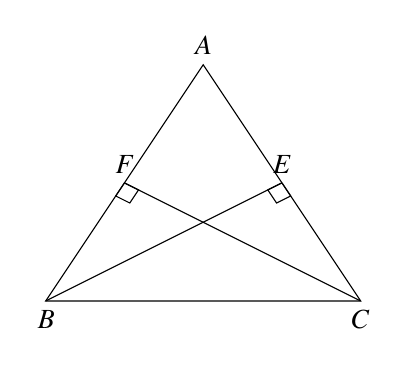
\begin{tikzpicture} 
        \coordinate (A) at (2, 3) {};
        \coordinate (B) at (0, 0) {};
        \coordinate (C) at (4, 0) {};
        \coordinate (F) at (1, 1.5) {};
        \coordinate (E) at (3, 1.5) {};
\draw (A)node[above]{$A$}--(B)node[below]{$B$}--(C)node[below]{$C$}--cycle;
\draw (B)node[below]{}--(E)node[above]{$E$};
\draw (C)node[below]{}--(F)node[above]{$F$};
\tkzMarkRightAngle[size=.2](B,E,C);
\tkzLabelAngle[dist=.5](B,E,C){};
\tkzMarkRightAngle[size=.2](C,F,B);
\tkzLabelAngle[dist=.5](C,F,B){};
\end{tikzpicture}
}
\caption{Triangle with equal altitudes on two sides}
\label{myfig}
\end{figure}
Given:-\\
1) Altitudes are Equal means their magnitude are same
 \begin{align}
 	\norm{\vec{E} - \vec{B}} = \norm{\vec{F} - \vec{C}} \label{1}
 \end{align}
2) Altitude makes right angle at the base therefore $\cos 90 =0$ therefore  FC $\perp$ BF and EB $\perp$ CE where $\textbf{m}$ is the directional vectors.
\begin{align}
\textbf{m}_{FC} \textbf{m}_{BF} = 0 \label{2}\\
\textbf{m}_{EB} \textbf{m}_{CE} = 0 \label{3}
\end{align}
From \eqref{2}
\begin{align}
    \brak{\vec{B}-\vec{F}}^T\brak{\vec{F}-\vec{C}}=\vec{0} && \brak{\vec{F}-\vec{C}}^T\brak{\vec{B}-\vec{F}}=\vec{0}\label{4}
\end{align}
From \eqref{2} and using \eqref{4} 
\begin{align}
    \brak{\vec{B}-\vec{C}}^T\brak{\vec{B}-\vec{C}}\\
    =\brak{\vec{B}-\vec{F}+\vec{F}-\vec{C}}^T\brak{\vec{B}-\vec{F}+\vec{F}-\vec{C}})
    \end{align}
    \begin{align}
      =\brak{\vec{B}-\vec{F}}^T\brak{\vec{B}-\vec{F}}+\brak{\vec{F}-\vec{C}}^T\brak{\vec{F}-\vec{C}} 
    \end{align}
\begin{align}
   \norm{\vec{B}-\vec{C}}^2=\norm{\vec{B}-\vec{F}}^2+\norm{\vec{F}-\vec{C}}^2\label{8} 
    \end{align}
    Similarly\\
    From \eqref{3}
    \begin{align}
        \brak{\vec{E}-\vec{B}}^T\brak{\vec{E}-\vec{C}}=\vec{0} && \brak{\vec{E}-\vec{C}}^T\brak{\vec{B}-\vec{E}}=\vec{0}\label{9}
        \end{align}
From  \eqref{3} and using \eqref{9}  
\begin{align}
    \brak{\vec{B}-\vec{C}}^T\brak{\vec{B}-\vec{C}}\\
    =\brak{\vec{B}-\vec{E}+\vec{E}-\vec{C}}^T\brak{\vec{B}-\vec{E}+\vec{E}-\vec{C}}
    \end{align}
    \begin{align}
      =\brak{\vec{B}-\vec{E}}^T\brak{\vec{B}-\vec{E}}+\brak{\vec{E}-\vec{C}}^T\brak{\vec{E}-\vec{C}} 
    \end{align}
\begin{align}
   \norm{\vec{B}-\vec{C}}^2=\norm{\vec{B}-\vec{E}}^2+\norm{\vec{E}-\vec{C}}^2\label{13}
    \end{align}        
    Equating \eqref{8} and \eqref{13} and using \eqref{1}
    \begin{align}
      \norm{\vec{B}-\vec{F}}^2+\norm{\vec{F}-\vec{C}}^2 = \norm{\vec{B}-\vec{E}}^2+\norm{\vec{E}-\vec{C}}^2  
    \end{align}
    \begin{align}
       \norm{\vec{B}-\vec{F}}^2=\norm{\vec{E}-\vec{C}}^2\\
       =\norm{\vec{B}-\vec{F}}=\norm{\vec{E}-\vec{C}}\label{16}
    \end{align}
Let $\angle FBC=\theta_1$  and  $\angle EBC=\theta_2$
    \begin{align}
        \brak{\vec{B}-\vec{F}}^T\brak{\vec{B}-\vec{C}}=\norm{\vec{B}-\vec{F}}\norm{\vec{B}-\vec{C}}\cos\theta_1\\
        \cos{\theta_1}=\frac{\brak{\vec{B}-\vec{F}}^T\brak{\vec{B}-\vec{C}}}{\norm{\vec{B}-\vec{F}}\norm{\vec{B}-\vec{C}}}\\
        \cos{\theta_1}=\frac{\brak{\vec{B}-\vec{F}}^T\brak{\vec{B}-\vec{F}+\vec{F}-\vec{C}}}{\norm{\vec{B}-\vec{F}}\norm{\vec{B}-\vec{C}}}\\
        \cos{\theta_1}=\frac{\brak{\vec{B}-\vec{F}}^T\brak{\vec{B}-\vec{F}} +\brak{\vec{B}-\vec{F}}^T\brak{\vec{F}-\vec{C}}}{\norm{\vec{B}-\vec{F}}\norm{\vec{B}-\vec{C}}}
        \end{align}
        From \eqref{4}
        \begin{align}
          \cos{\theta_1}=\frac{\brak{\vec{B}-\vec{F}}^T\brak{\vec{B}-\vec{F}}}{\norm{\vec{B}-\vec{F}}\norm{\vec{B}-\vec{C}}} \\
          \cos{\theta_1}=\frac{\norm{\vec{B}-\vec{F}}^2}{\norm{\vec{B}-\vec{F}}\norm{\vec{B}-\vec{C}}}\\
          \cos{\theta_1}=\frac{\norm{\vec{B}-\vec{F}}}{\norm{\vec{B}-\vec{C}}}
        \end{align}
        Similarly for $\angle EBC=\theta_2$
       \begin{align}
        \brak{\vec{C}-\vec{E}}^T\brak{\vec{B}-\vec{C}}=\norm{\vec{C}-\vec{E}}\norm{\vec{B}-\vec{C}}\cos\theta_2\\
        \cos{\theta_2}=\frac{\brak{\vec{C}-\vec{E}}^T\brak{\vec{B}-\vec{C}}}{\norm{\vec{C}-\vec{E}}\norm{\vec{B}-\vec{C}}}\\
        \cos{\theta_2}=\frac{\brak{\vec{C}-\vec{E}}^T\brak{\vec{B}-\vec{E}+\vec{E}-\vec{C}}}{\norm{\vec{C}-\vec{E}}\norm{\vec{B}-\vec{C}}}\\
        \cos{\theta_2}=\frac{\brak{\vec{C}-\vec{E}}^T\brak{\vec{B}-\vec{E}} +\brak{\vec{C}-\vec{E}}^T\brak{\vec{E}-\vec{C}}}{\norm{\vec{C}-\vec{E}}\norm{\vec{B}-\vec{C}}}
        \end{align}
        From {\eqref{9}}
        \begin{align}
          \cos{\theta_2}=\frac{\brak{\vec{C}-\vec{E}}^T\brak{\vec{C}-\vec{E}}}{\norm{\vec{C}-\vec{E}}\norm{\vec{B}-\vec{C}}} \\
          \cos{\theta_2}=\frac{\norm{\vec{C}-\vec{E}}^2}{\norm{\vec{C}-\vec{E}}\norm{\vec{B}-\vec{C}}}\\
          \cos{\theta_2}=\frac{\norm{\vec{C}-\vec{E}}}{\norm{\vec{B}-\vec{C}}}
        \end{align}
        From \eqref{16} we know $\norm{\vec{B}-\vec{F}}=\norm{\vec{E}-\vec{C}}$ we conclude
        \begin{align}
            \cos\theta_1=\cos\theta_2
            \implies\theta_1=\theta_2
        \end{align}
        So the sides opposite to equal angles are equal. Hence AB=AC hence the given Triangle is isosceles.
    \end{document}